\scanpage{65}
\mspage{28}
\uline{12} Récapitulation (des données de déploiement,
relatif à un ens ordonné $I$, fini disons\ldots)

\[
\left\{\begin{aligned}
\text{a) }&\text{Espaces }\Sigma_i\quad(i\in I)\\
\text{b) }&\text{Espaces }\Sigma_{i,j}\quad(i<j,\ i,j\in I)\\
\text{c) }&\text{Applications }\Sigma_{i,j}\xrightarrow{s_{ij}}\Sigma_i,\quad
\Sigma_{ij}\xrightarrow{b_{ij}}\Sigma_j
\end{aligned}\right.
\]
\margin{C'est la structure envisagée dans le Scholie (p. $26/27$)
plus une application continue strictement croissante
$\Sigma\overset{\varphi}{\unsure{-|\longrightarrow}}I$, telle que
$\forall x\in\Sigma$, $\varphi|\Sigma_{<x}$ soit injective
(\uline{donc} la relation d'ordre de
\inserted{\unsure{(pour $i$ ?)}} $\Sigma_{<x}$
soit induite par celle de $I_{<i}$)}

Conditions

a) $\Sigma_{ij}\longrightarrow\Sigma_j$
\deleted{\unsure{immersion}}\inserted{plongement} fermé
\deleted{bordant}
\inserted{[On identifie $\Sigma_{ij}$ à un ss-espace fermé de
$\Sigma_j$ par $b_{ij}$]}

b) $\Sigma_{i,k}\cap\Sigma_{j,k}=\varnothing$ si $i,j$,
\deleted{$\unsure{\exists}$} non comparables
\deleted{\unsure{(on suppose|(on supp}}
\unsure{\inserted{\deleted{\unsure{($i<j$)}}}|\deleted{\unsure{($i<j$)}}}
(NB $i,j<k$)
\margin{\uline{NB} La condition \uline{b}) équivaut à celle
que dans l'ens ordonné $\Sigma=\coprod\Sigma_i$, les ensembles
$\Sigma_{<x}$ sont tot$ {}^t$ ordonnés}

c) Pour $\unsure{\deleted{\unsure{i}}|\unsure{i}}\ i<j<k$ posons
\[
\Sigma_{ijk}=\Sigma_{ik}\cap\Sigma_{jk}
\uline{\subset\unsure{\Sigma_k}}.
\]
On a alors \inserted{dans $\Sigma_{jk}$ :}
\deleted{$\unsure{\Sigma_{jk}}$}
\diagram{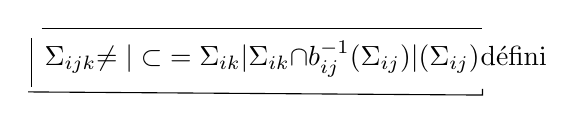
\begin{tikzpicture}[baseline=(eq.base)]
\node[anchor=base west,inner sep=0pt] (eq) at (0,0)
{$\Sigma_{ijk}\deleted{\unsure{\ne|\subset}}=
\deleted{\unsure{\Sigma_{ik}|\Sigma_{ik}\cap}}
b_{ij}^{-1}\unsure{(\Sigma_{ij})|\deleted{(\Sigma_{ij})}}$};
\node[anchor=base west,inner sep=0pt] at (eq.base east)
{\deleted{\unsure{défini}}};
\draw ([xshift=-.03cm,yshift=.16cm]eq.north west)
-- ([xshift=.03cm,yshift=.16cm]eq.north east);
\draw ([xshift=-.16cm,yshift=.03cm]eq.north west)
-- ([xshift=-.16cm,yshift=-.12cm]eq.south west);
\draw ([xshift=-.20cm,yshift=-.18cm]eq.south west)
-- ([xshift=.03cm,yshift=-.22cm]eq.south east)
-- ([xshift=.03cm,yshift=-.14cm]eq.south east);
\end{tikzpicture}}
\deleted{\unsure{une}}

On a donc, pour $i<j<k$, un diagramme
commutatif hexagonal
\diagram{\begin{tikzpicture}[x=1.15cm,y=1.15cm]
\node (I) at (0,0) {$\Sigma_i$};
\node (IK) at (1.7,1.6) {$\Sigma_{ik}$};
\node (K) at (4.2,1.6) {$\Sigma_k$};
\node (IJK) at (2.7,.1) {$\Sigma_{ijk}$};
\node (JK) at (5.7,.1) {$\Sigma_{jk}$};
\node (IJ) at (1.7,-1.4) {$\unsure{\Sigma}_{ij}$};
\node (J) at (4.2,-1.4) {$\Sigma_j$};
\node at (-1.5,.05) {(41)};
\draw[->] (1.24,1.23)--(.43,.43);
\node at (.64,1.05) {$s_{ik}$};
\draw[->] (2.30,1.75)
..controls (2.05,1.65) and (2.06,1.47)..(2.31,1.47)
--(3.52,1.47);
\node at (2.91,1.95) {$b_{ik}$};
\draw[->] (5.10,.65)
..controls (5.50,.45) and (5.50,.82)..(4.77,1.27);
\node at (5.54,1.06) {$b_{jk}$};
\draw[->] (2.30,.68)
..controls (2.65,.48) and (2.64,.82)..(2.07,1.20);
\draw[->] (3.28,.28)
..controls (3.03,.17) and (3.04,.02)..(3.27,.02)
--(4.97,.02);
\draw[->] (2.36,-.28)--(1.98,-.94);
\draw[->] (1.24,-1.12)--(.43,-.43);
\node at (.63,-1.07) {$s_{ij}$};
\draw[->] (2.40,-1.23)
..controls (2.13,-1.36) and (2.13,-1.51)..(2.39,-1.51)
--(3.53,-1.51);
\node at (2.97,-1.97) {$b_{ij}$};
\draw[->] (5.18,-.29)--(4.65,-1.12);
\node at (5.21,-.84) {$s_{jk}$};
\node at (3.57,.86) {cart};
\node at (3.64,-.71) {cart};
% Two detached ink points, without assigned mathematical function.
\fill (2.34,-1.97) circle (.012);
\fill (2.39,-1.91) circle (.012);
\end{tikzpicture}}

où les flèches $\lhook\joinrel\relbar\joinrel\relbar$ sont des inclusions
fermees \inserted{cf plus bas} (bordantes), et les flèches
\(\mathrel{\begin{tikzpicture}[baseline=-.35ex,x=1cm,y=1cm]
\draw[->] (0,0)--(1.2,0);
\fill (.45,.55) circle (.016);
\end{tikzpicture}}\)
sont des applications qui seront fibrantes et propres
dans le cas équisingulier.
\margin{\handwritten{64}}
